\documentclass[main]{subfiles}

\begin{document}

\chapter{GPS - Test 2}
\label{chap-gps-test-2}

\section{Objetivos}
%\ref{} agregar refs
%TODO esta ref es trucha! cambiar por la posta!!
\label{chap-gps-test-1}

En el capítulo anterior se comenzó a analizar la performance del GPS. Se intentó reconstruir un polígono, y se analizó el error al estimar la posición de un punto fijo. En este capítulo se continúa dicho análisis, repitiendo el procedimiento, pero con un polígono más grande, y tiempo más largos para la estimación de la posición de un punto fijo.

\section{Materiales}

\begin{itemize}
\item GPS.
\item Laptop.
\item Trípode (de fotografía).
\item Cinta métrica, pintura y cuerda.
\end{itemize}

\newpage
\section{Procedimiento}
\label{sec:gps2-procedimiento}

En esta prueba se trata de obtener el error del GPS en el plano paralelo a la tierra, es decir, el error en latitud y longitud.

El experimento que se diseñó consiste en marcar un rectángulo sobre el suelo (pasto), utilizando 6 puntos, con la siguiente disposición:

\begin{quote}
\begin{quote}
\begin{verbatim}
      Árbol              
 Árbol               Árbol
           Gente_q_me_va_a_afanar
      Árbol
 -- < -- < -- < -- < -- < -- < -- <
    calle que sube de la rambla
 -- > -- > -- > -- > -- > -- > -- > 
 3                2                1
 x ---- ---- ---- x ---- ---- ---- x
 |                                 |      Orientación del GPS:
 |                                 |            led
 |                                 |             ^
 |                                 |             |
 |                                 |             |
 x ---- ---- ---- x ---- ---- ---- x            usb
 6                5                4

     Estacionamiento de la facultad
\end{verbatim}
\end{quote}
\end{quote}

A diferencia del experimento de la sección \ref{chap-gps-test-1}, aqui todas líneas punteadas son de 6m de largo, en lugar de 1m. Resulta en un rectángulo de 6m por 12m.

Los pasos a seguir son los siguientes:

\begin{enumerate}
\item Construir el rectángulo sobre un superficie plana.
  \begin{itemize}
  \item Se utilizó pintura para marcar los vértices del triángulo.
  \item Para trazar uno de los lados de 12 metros (puntos 1,2 y 3), se fijó una cuerda de 12 metros (con el punto medio marcado) a un punto, y se extendió (sin estirarla). El principio (\verb+1+) y el final (\verb+3+) de la cuerda son vértices del polígono, y el punto medio (\verb+2+) es otro de los puntos de interés.
  \item Para construir rectas perpendiculares se utilizó una cuerda de 6m, y otra de 8.5m\footnote{Pitágoras: $8.5 \approx \sqrt{6^2 + 6^2} = 8.4852...$}. Uno de los extremos de la cuerda de 6 metros se fijó al \verb+1+, y uno de los extremos de la cuerda de 8.5m se fijó a \verb+2+. El punto donde ambas se intersectan corresponde a \verb+4+. Un procedimiento similar se siguió para determinar la ubicación de \verb+5+ y \verb+6+.
  \end{itemize}
\item Medir, con un metro, las distancias entre todos los puntos.
\item Utilizar mínimos cuadrados para minimizar el error entre las distancias esperadas, y las experimentales. Esto puede llevar a trabajar con un polígono que \textbf{no} sea un rectángulo, pero el error será menor que el que resultaría de usar los valores teóricos.
\item Fijar la altura y la orientación del GPS, y tomar medidas en cada uno de los puntos \verb+[1,2,3,4,5,6]+.
\item Tomar un punto como origen, y comparar la figura que resulta de los datos provenientes del GPS con las medidas tomadas con el metro.
\end{enumerate}

En la figura \ref{fig:tripode_con_plomada.jpg} se observa el trípode que sostiene al GPS. El objetivo era tener el GPS a una altura fija, y separado del piso. Al nivel del piso los rebotes degradan seriamente la performance del GPS. La cuerda que marca el lado del polígono, junto con las patas del trípode, se utilizaron para fijar la orientación del GPS durante el experimento.

\begin{figure} [h!]
  \centering
  \subfloat[Trípode de fotografía, con el GPS atado en lugar de la cámara..]{\label{fig:tripode_con_plomada.jpg}
  		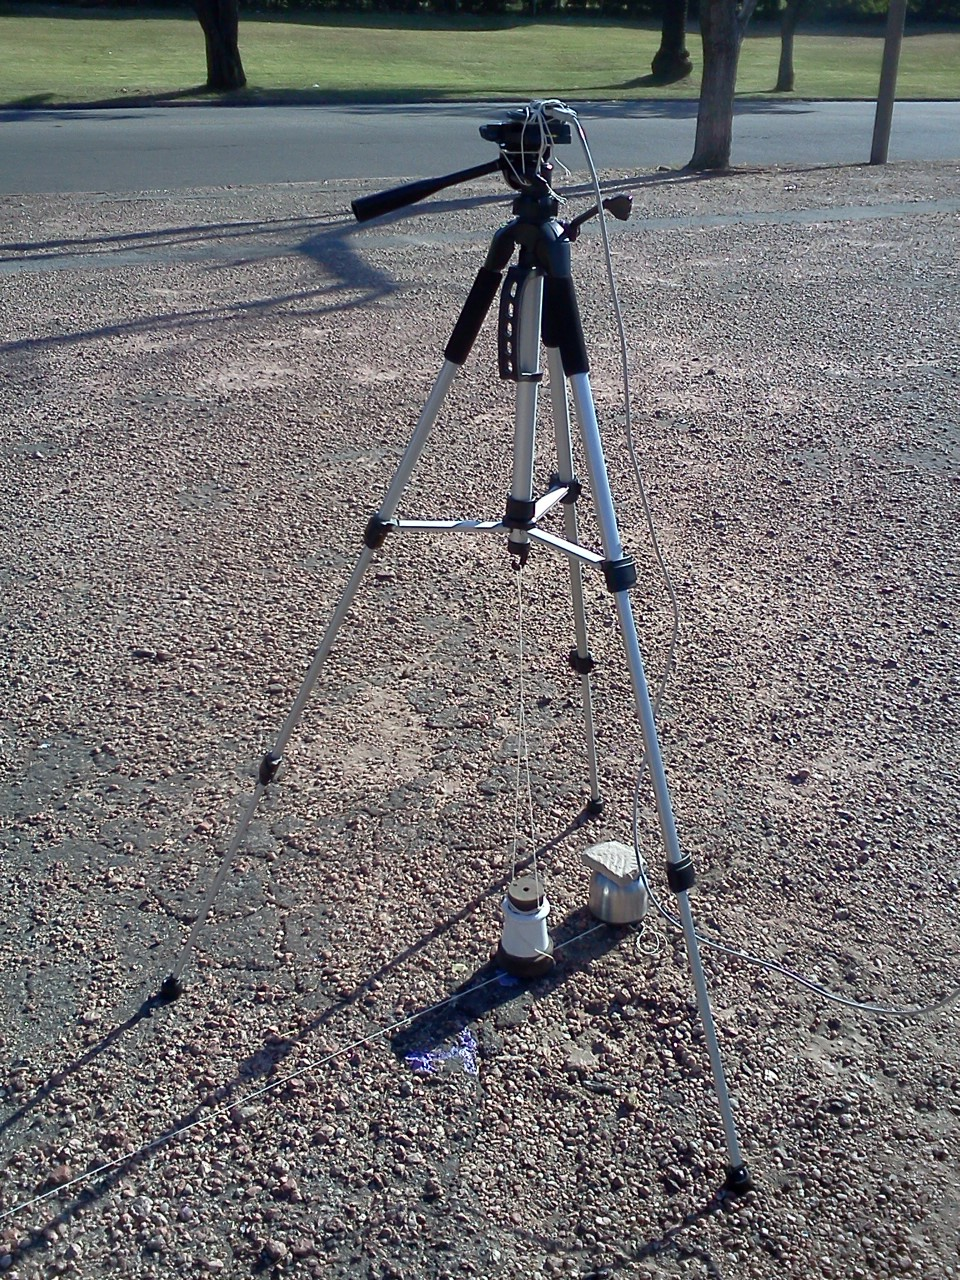
\includegraphics[width=0.45\textwidth]{./pics_gps/tripode_con_plomada.jpg}}
  \subfloat[GPS amarrado al trípode.]{\label{fig:vista_usb.jpg}
  		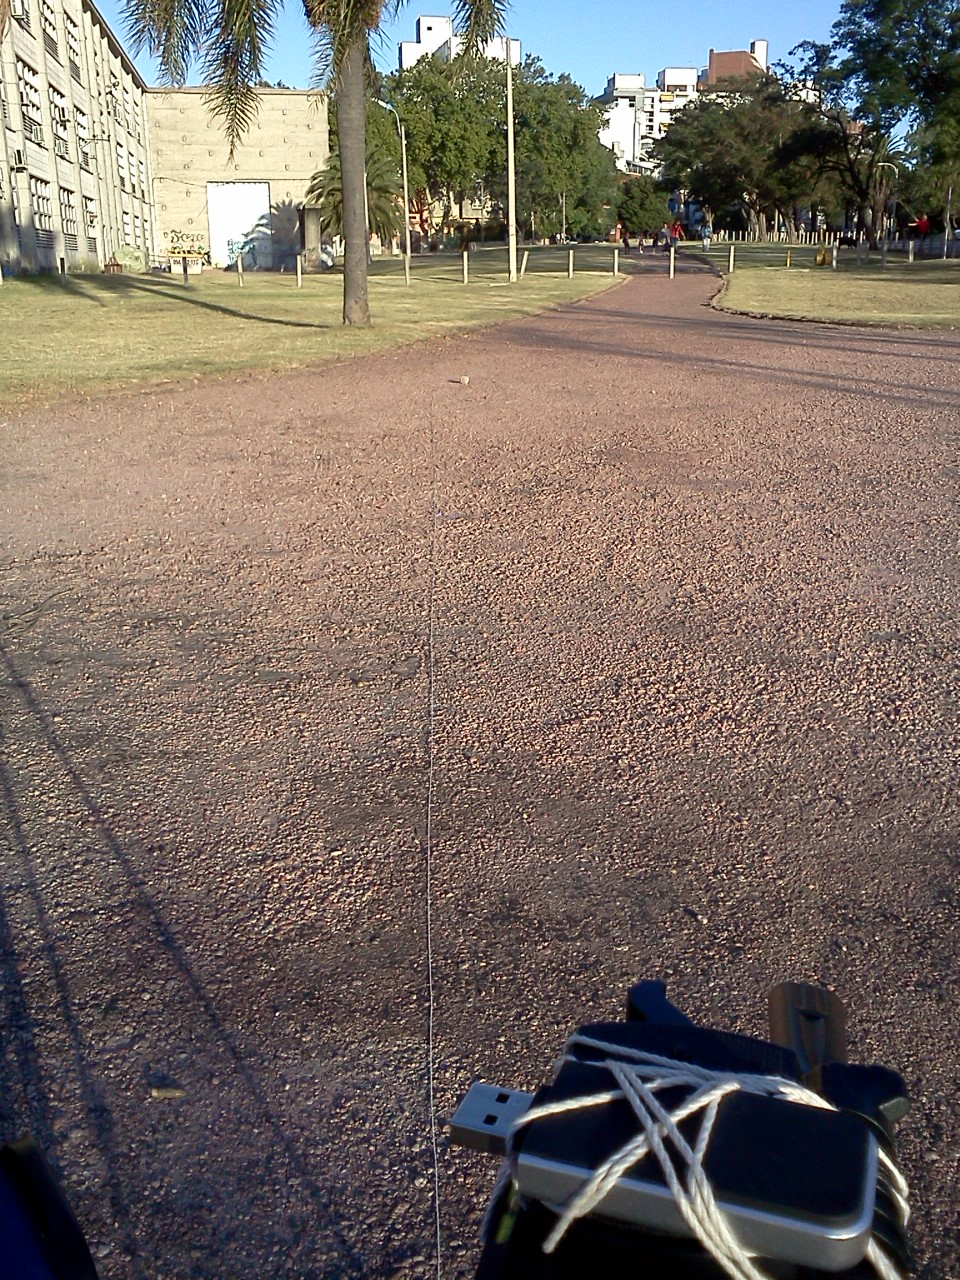
\includegraphics[width=0.45\textwidth]{./pics_gps/vista_usb.jpg}}
  \caption{GPS + Atril}
  \label{fig:rebotes}
\end{figure}

\newpage
\subsection{Adquisición de datos}
\label{sec:adquisicion-de-datos}

Para tomar datos se conectó el GPS, que manda información mediante USB-serie, al puerto USB de una computadora. En la computadora se utilizó el \href{http://catb.org/gpsd/}{GPSD}, un software open-source que hace de \textit{daemon}, y se encarga de transformar lo que llega del GPS en una estructura de datos fácil de manejar en \verb+C+.

El GPS emite sentencias NMEA a través de USB serie, a 38400bps. Trabaja con sentencias:
\begin{itemize}
\item GPGGA - \textit{Global Positioning System Fix Data}: Información sobre la fecha, posición y datos relevantes sobre el \textit{fix}.
\item GPGSV - \textit{Satellites in view}: Información sobre la cantidad de satélites detectados, y la calidad de la señal proveniente de cada uno.
\item GPGSA - \textit{DOP and active satellites}: Información sobre DOP\footnote{\textit{Dilution of precision}.} y satélites activos.
\item GPRMC - \textit{Recommended minimum specific GPS/Transit data}: Sentencia mínima recomendada, trae suficiente información como para poder trabajar con el GPS.
\item GPVTG - \textit{Track Made Good and Ground Speed}: Información sobre la dirección y la velocidad (\textbf{no} sobre la posición absoluta).
\end{itemize}

\section{Geometría: DOP - \textit{Dilution of precision}}
\label{sec:dop}

\begin{wrapfigure}{r}{0.5\textwidth}
\vspace{-30pt}
  \begin{center}
    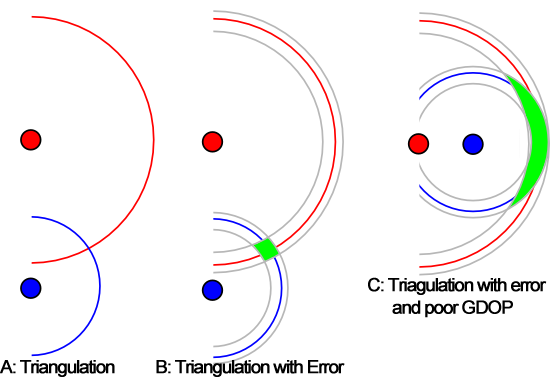
\includegraphics[width=.5\textwidth]{./pics_gps/dop.png}
  \end{center}
\vspace{-20pt}
  \caption{DOP en 2 dimensiones.}
\vspace{-50pt}
\label{fig:dop.png}
\end{wrapfigure}

El método que utiliza el GPS para determinar su ubicación consiste básicamente en:
\begin{enumerate}
\item Determinar la distancia $r_i$ a cada satélite $S_i$, cuya posición es $P_i$.
\item Repetir el paso anterior para cada satélite disponible.
\item Intersectar las ``cáscaras'' de las esferas de centros $P_i$ y radios $r_i$.
\end{enumerate}

Las ``cáscaras'' de las esferas no serán de ancho despreciable, ya que hay un cierta incertidumbre asociado a los datos. Esto implica que la intersección será un volumen, en lugar de un punto. La geometría de la distribución de los satélites determinará el tamaño de este volumen, y por lo tanto la incertidumbre en la determinación de la posición. En la figura \ref se muestra un ejemplo ilustrativo, en dos dimensiones.

El DOP es el cociente entre la exactitud de la ubicación y exactitud de la medida\cite{bib:sat-pos}:
\begin{equation*}
  \sigma = \sigma_o.DOP
\vspace{-10pt}
\end{equation*}
donde
\begin{itemize}
\item $\sigma$: Exactitud de la medida.
\item $\sigma_o$: Exactitud de la posición. 
\end{itemize}

 Básicamente, el DOP representa la sensibilidad de localización frente a errores en las medidas, o sea, cuanto te vas a perder si te llego una medida equivocada. Cuanto más bajo sea el DOP, mejor. En la tabla \ref{tab:dop} se muestra como interpretar valores típicos\cite{bib:sat-dop-values}.

\begin{table}[H]
\begin{center}
\begin{tabular}{|l|c||p{7cm}|}
\hline
\rowcolor[gray]{0.9}
1 & Ideal & Máxima exactitud posible.\\
\rowcolor[gray]{0.95}
1-2 & Excelente & La exactitud a este nivel se considera suficiente para casi cualquier aplicación.\\
\rowcolor[gray]{0.9}
2-5 & Bueno & Este nivel marca el mínimo apropiado para navegación. \\
\rowcolor[gray]{0.95}
5-10 & Moderado & Las medidas se pueden utilizar, pero es recomendado buscar un lugar con cielo más abierto. \\
\rowcolor[gray]{0.9}
10-20 & Regular & Solo se deben usar los datos para estimaciones de muy poca precisión. \\
\rowcolor[gray]{0.95}
$>$20 & Malo & A este nivel, las exactitud de las medidas puede tener un error de hasta 300m, deben descartarse. \\
\hline
\end{tabular}
\caption{Interpretación de los valores de DOP.}
\label{tab:dop}
\end{center}
\end{table}

El GPS envía información sobre:
\begin{itemize}
\item \textit{HDOP} - DOP horizontal:
  \begin{equation}
    \label{eq:hdop}
    HDOP = \sqrt{\sigma_{easting}^2+\sigma_{northing}^2}    
  \end{equation}
\item \textit{VDOP} - DOP vertical:
  \begin{equation}
    \label{eq:vdop}
    VDOP = \sqrt{\sigma_{altitud}^2}
  \end{equation}
\item \textit{PDOP} - DOP de la posición:
  \begin{equation}
    \label{eq:pdop}
    PDOP = \sqrt{\sigma_{easting}^2+\sigma_{northing}^2 + \sigma_{altitud}^2}
  \end{equation}
\end{itemize}

Esta información se puede utilizar en el algoritmo de control, para ponderar los datos provenientes del GPS.

\newpage
\subsection{Verificación del polígono}
\label{sec:verificacion-del-poligono}

Una vez construido el polígono, es de interés medir todas las diagonales (con la cinta métrica) por dos motivos:
\begin{itemize}
\item Verificar que no se cometieron errores.
\item Hacer mínimos cuadrados con las medidas, de manera de obtener un polígono, que no tiene porqué ser (y en general no será) un rectángulo, sino algo similar a un rectángulo, más ajustado a la realidad.
\end{itemize}

Las medidas tomadas se resumen en la tabla \ref{tab:diagonales-poligono}, donde \verb+D12+ representa la medida de la recta que une el punto \verb+1+ con el punto \verb+2+, en cm.

\begin{table}[H]
\begin{center}
\begin{tabular}{|c|c|c|c|c|}
\hline
\rowcolor[gray]{0.9}
\textbf{D12} & \textbf{D13} & \textbf{D14} & \textbf{D15} & \textbf{D16} \\
\hline
603 & 1205 & 606 & 855 & 1345 \\
\hline
\rowcolor[gray]{0.9}
\textbf{D23} & \textbf{D24} & \textbf{D25} & \textbf{D26} & \textbf{D34} \\
\hline
603 & 853 & 608 & 853 & 1344\\
\hline
\rowcolor[gray]{0.9}
\textbf{D35} & \textbf{D36} & \textbf{D45} & \textbf{D46} & \textbf{D56} \\
\hline
850 & 602 & 602 & 1202 & 603 \\
\hline
\end{tabular}
\caption{Diagonales del polígono en cm.\\\textbf{Lectura}: \textbf{D24} representa la longitud (en cm) de la recta que une el punto $2$ con el punto $4$.}
\label{tab:diagonales-poligono}
\end{center}
\end{table}

\begin{wrapfigure}{r}{0.6\textwidth}
  \begin{center}
    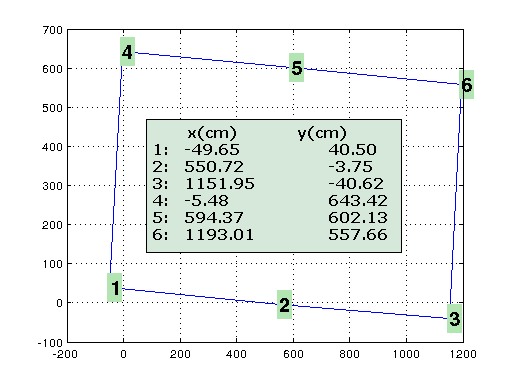
\includegraphics[width=.5\textwidth]{./pics_gps/pol_mc.png}
  \end{center}
  \caption{Polígono luego de MC.}
\label{fig:pol_mc.png}
\end{wrapfigure}

El polígono resultante se observa en la figura \ref{fig:pol_mc.png}. El error relativo, es decir, el cociente entre las medidas de cada recta \textbf{D\#\#} resultante de aplicar MC, y lo esperado en el polígono teórico, de 6m de lado, es:

\begin{itemize}
\item $9.51\%$ en el peor caso.
\item $4.65\%$ en promedio.
\end{itemize}

Se considera que el error, siendo  menor al 10\% en el peor caso, es aceptable.

En realidad se podría hacer una figura irregular cualquiera, y tomarlo en cuanto en el resto del experimento, pero complicaría la interpretación intuitiva de los resultados.

\newpage
\subsection{Punto fijo - 10 minutos}
\label{sec:gps2-punto-fijo-10-minutos}

Se tomaron datos durante 10 minutos ($\approx$ 600 muestras) en cada uno de los vértices del polígono, con el objetivo de observar la estabilidad de la información proveniente del GPS.

En la figura \ref{fig:10min_grid.png} se muestran los datos luego de restar el promedio, o sea que se muestra el error respecto al valor promedio.

\begin{figure}[h!]
  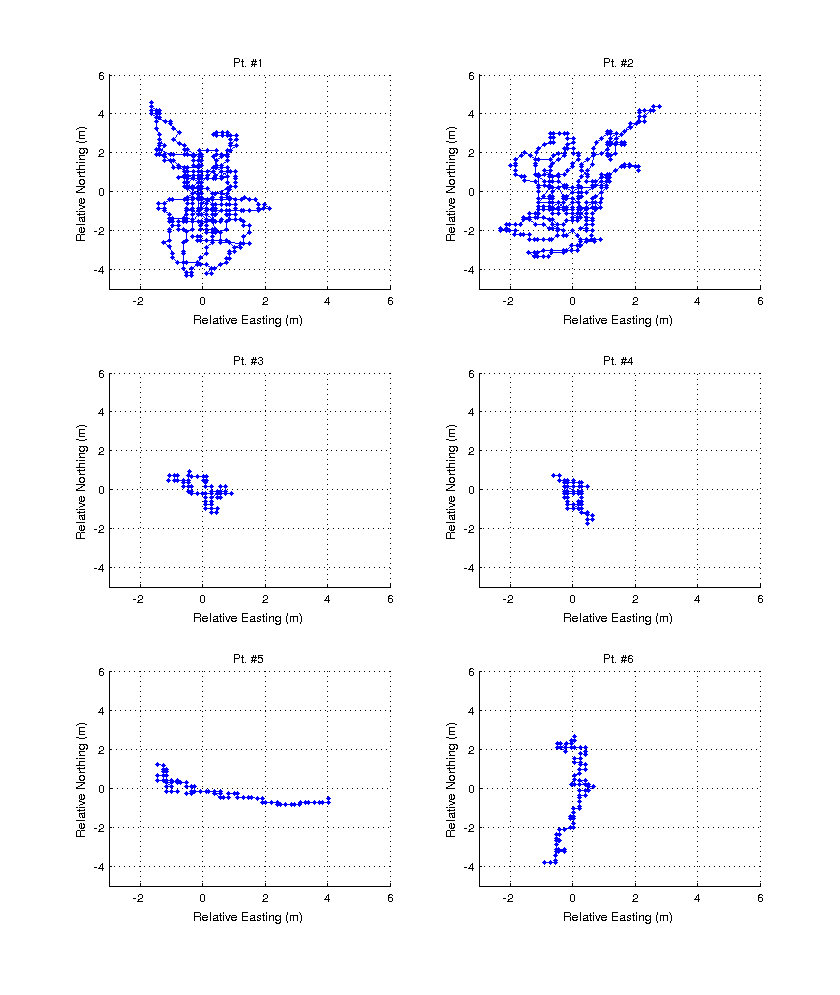
\includegraphics[width=0.8\textwidth]{./pics_gps/10min_grid.png}
  \caption{GPS quieto en cada punto del polígono, GPS orientado como se describe en \ref{sec:gps2-procedimiento} y se muestra en \ref{fig:vista_usb.jpg}.}
  \label{fig:10min_grid.png}
\end{figure}

Cabe destacar que en la figura \ref{fig:10min_grid.png} no parece haber la misma cantidad de muestras por punto, pese a que en el log habían aproximadamente la misma cantidad de datos por punto. Esto se debe a que a veces en el log se genera información repetida, es decir, el GPS envía sucesivamente la misma información, y la etiqueta como \textit{información válida}. Esto se analiza con más detalle en la sección \ref{sec:tasa-de-muestreo}.

\newpage
En la figura \ref{fig:10m_todos.png} se observan todas las gráficas de la figura \ref{fig:10min_grid.png}, pero superpuestas.

Si el GPS fuese perfecto, entonces todas las muestras coincidirían con el promedio, y estarían ubicadas en el punto \verb+[0,0]+. El círculo negro tiene 2.5m de radio, las muestras que caen fuera de él están a más de 2.5m del valor promedio. En la leyenda se muestra qué porcentaje de las muestras caen fuera del círculo.

\begin{figure}[h!]
  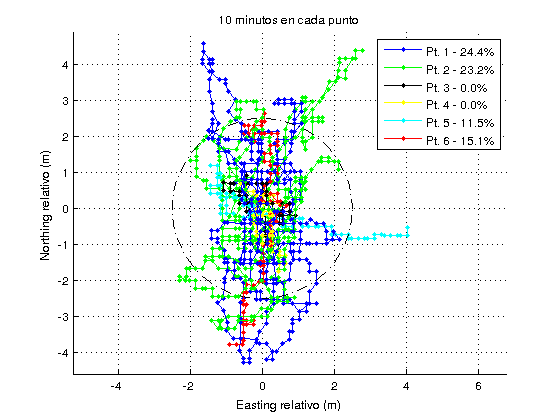
\includegraphics[width=1.1\textwidth]{./pics_gps/10m_todos.png}
  \caption{Error respecto al valor medio (Plots de \ref{fig:10min_grid.png} superpuestos). En la leyenda se muestran que porecentaje de muestras que caen a más de 2.5m del promedio.}
  \label{fig:10m_todos.png}
\end{figure}

\newpage
\subsection{Punto fijo - 2 minutos}
\label{sec:gps2-punto-fijo-2-minutos}

Se repitió el experimento, tomando 2 minutos de muestras por punto. Se optó por tomar datos durante solamente 2 minutos para agilizar el experimento, y acercarse más a un tiempo razonable. Los resultados fueron similares a los que se obtuvieron con el experimento de 10 minutos.

Se orientó el GPS de 3 maneras distintas, siempre alineando el trípode con uno de los lados de 12m del rectángulo:

\begin{enumerate}
\item USB hacia la calle, LED hacia el estacionamiento, como en la figura \ref{fig:or3.jpg}.
\item USB hacia la rambla, LED hacia el IIE (no hay figura)
\item Como en la figura \ref{fig:or2.jpg}.
\item Nuevamente, USB hacia la calle, LED hacia el estacionamiento, como en la figura \ref{fig:or3.jpg}.
\end{enumerate}

\begin{figure} [h!]
  \centering
  \subfloat[Orientación \#3]{\label{fig:or2.jpg}
  		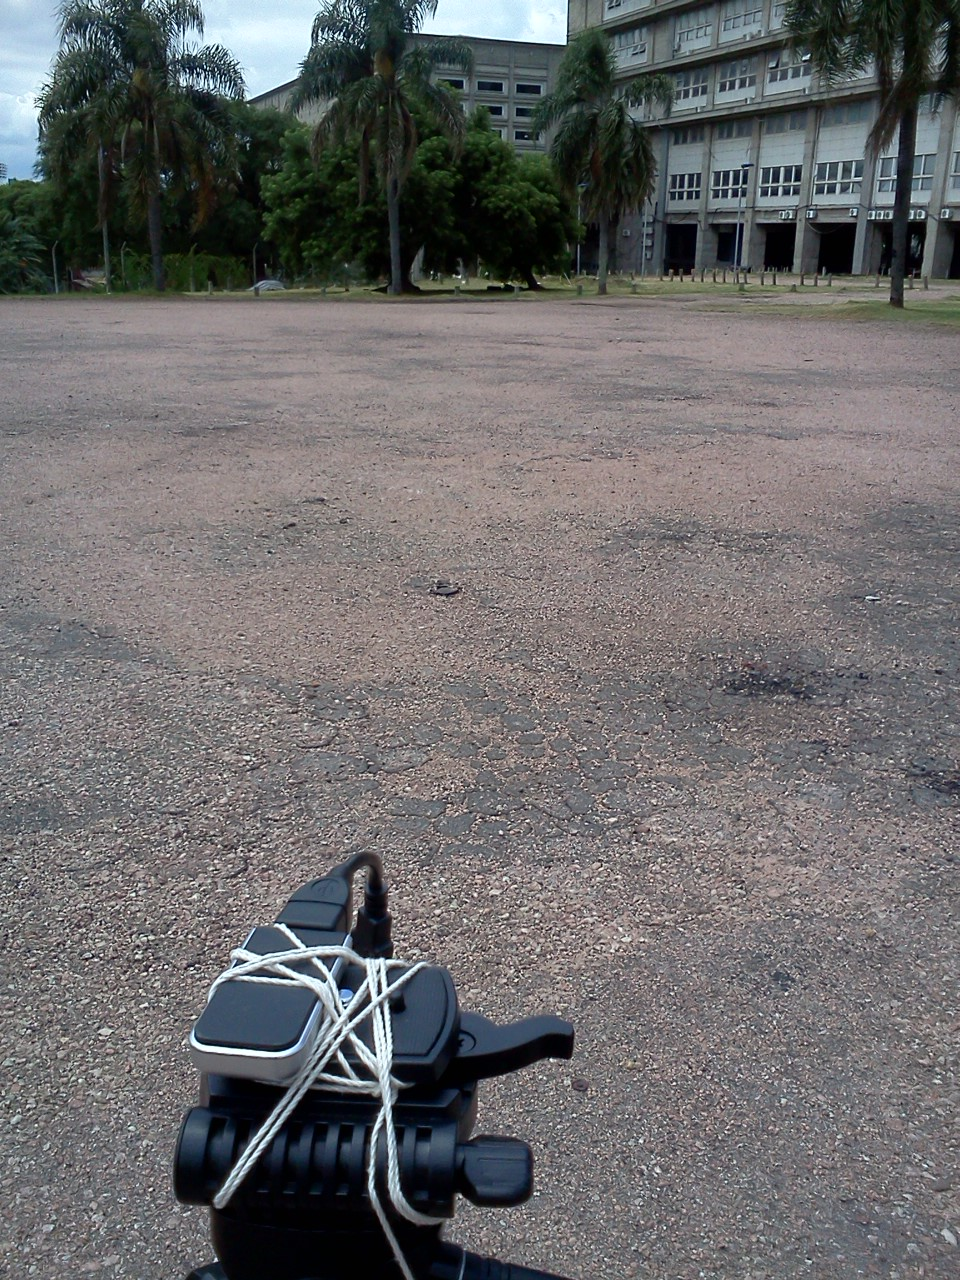
\includegraphics[width=0.45\textwidth]{./pics_gps/or2.jpg}}
  \subfloat[Orientación \#1 y \#4.]{\label{fig:or3.jpg}
  		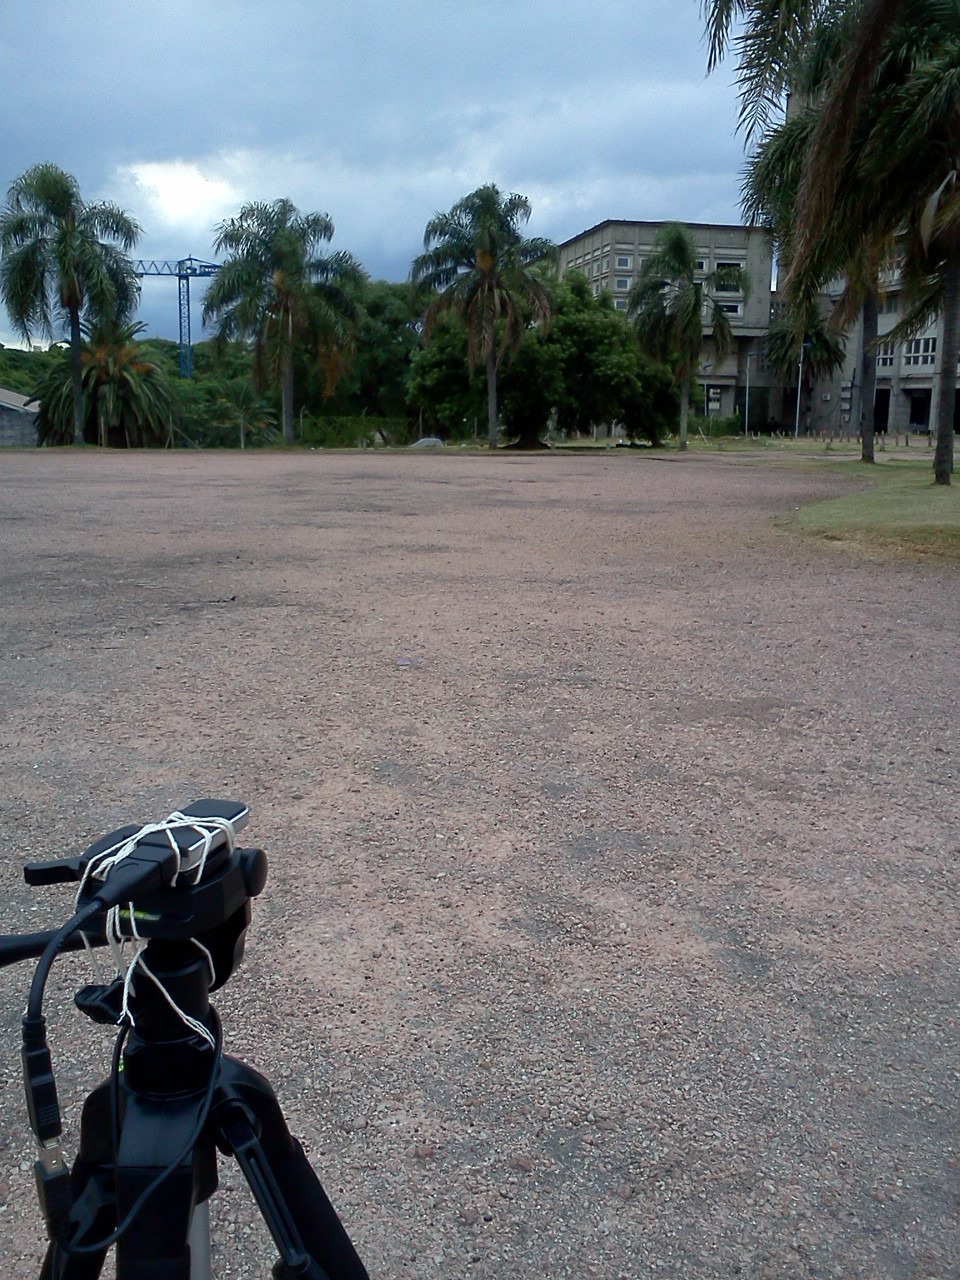
\includegraphics[width=0.45\textwidth]{./pics_gps/or3.jpg}}
  \caption{Fotos de algunas de las orientaciones del GPS en las pruebas de 2 minutos por punto.}
  \label{fig:or-2-m}
\end{figure}

Los resultados se observan en las siguientes figuras. Nuevamente, en la leyenda se muestra qué \textbf{porcentaje de las muestras caen a más de 2.5m del valor promedio}.

\newpage
\begin{figure}[h!]
  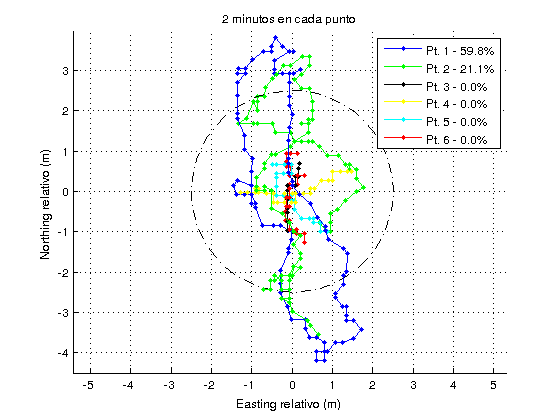
\includegraphics[width=.9\textwidth]{./pics_gps/2m_or1_todos.png}
  \caption{Orientación: \textbf{4}.}
\vspace{-30pt}
  \label{fig:2m_or1_todos.png}
\end{figure}

\begin{figure}[h!]
  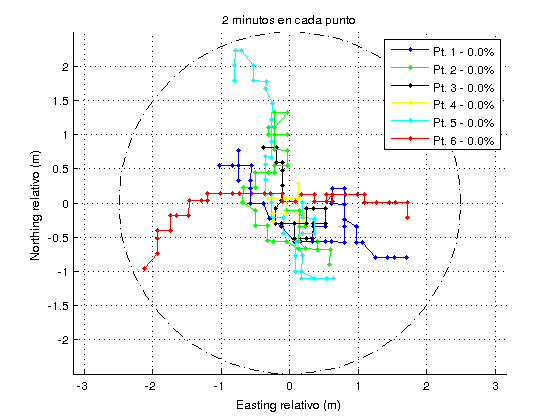
\includegraphics[width=1\textwidth]{./pics_gps/2m_or2_todos.png}
  \caption{Orientación: \textbf{2}.}
  \label{fig:2m_or2_todos.png}
\end{figure}

\newpage
\begin{figure}[h!]
  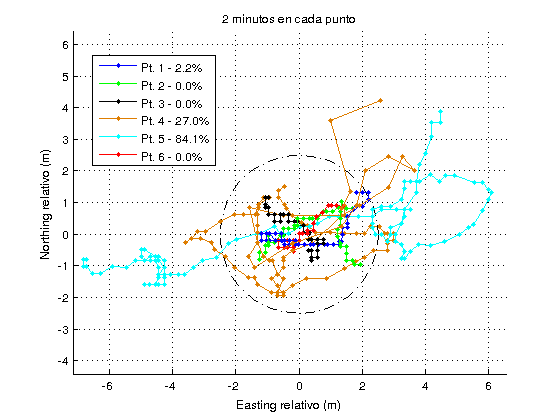
\includegraphics[width=1\textwidth]{./pics_gps/or2_todos_cut.png}
  \caption{Orientación: \textbf{3}.}
\vspace{-30pt}
  \label{fig:or2_todos_cut.png}
\end{figure}

\begin{figure}[h!]
  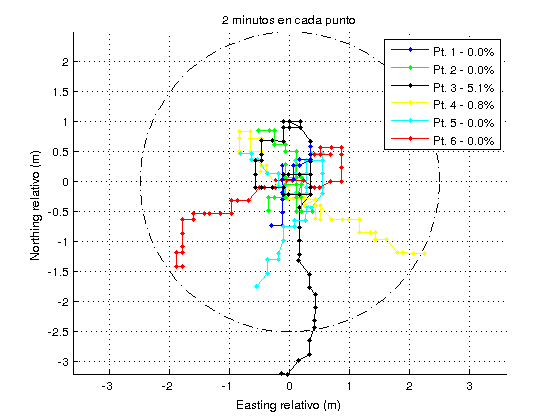
\includegraphics[width=.9\textwidth]{./pics_gps/or3_todos.png}
  \caption{Orientación: \textbf{4}}
  \label{fig:or3_todos.png}
\end{figure}

\newpage
\subsubsection{Punto fijo: Análisis}
\label{sec:gps2-punto-fijo-analisis}

\begin{itemize}
\item Influencia de la cantidad de \textbf{satélites disponibles}

La teoría dice que con 4 satélites debería alcanzar para obtener un \textit{fix 3D}, es decir, estimar la posición sobre la esfera terrestre, y la distancia (altura) a la misma. Se recomienda tener no menos de 6. Durante el experimento de la figura \ref{fig:or2_todos_cut.png}, en un momento el GPS perdió señal, y el número de satélites disponibles, que usualmente anda por los 9 o 10, pasó a ser 4. Los datos correspondientes se muestran en la figura \ref{fig:or2_todos_sat_mal.png}. El trazo naranja, con un error de hasta 23 metros, corresponde a instantes donde la cantidad de satélites era entre 4 y 5. Luego de volver a 9 o 10 satélites, los datos vuelven a ser más razonables.

\begin{figure}[h!]
  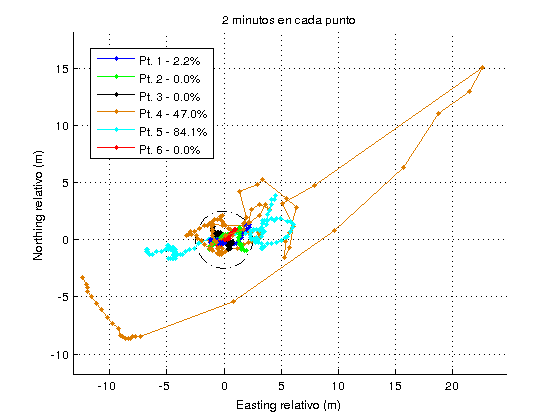
\includegraphics[width=1\textwidth]{./pics_gps/or2_todos_sat_mal.png}
  \caption{Datos con solamente 4 satélites. Orientación: \textbf{3}.}
  \label{fig:or2_todos_sat_mal.png}
\end{figure}

En la figura \ref{fig:or2_todos_cut.png} se observa el mismo log que en \ref{fig:or2_todos_sat_mal.png}, pero luego de haber quitado las muestras correspondientes al período donde se deterioró la señal.

No se pudo encontrar una explicación para la mala calidad de las muestras correspondientes al punto 5 en la figura \ref{fig:or2_todos_cut.png}. La cantidad de satélites disponibles se mantuvo estable en 9 o 10 durante la adquisición de esos datos.
\item Influencia de la \textbf{orientación}:

No parece haber una correlación directa entre resultados y la orientación del GPS, evidencia de esto son las figuras \ref{fig:or3_todos.png} y \ref{fig:2m_or1_todos.png}, que fueron tomadas con la misma orientación.

Resulta  intuitivo suponer que existe, debido a que el GPS tiene una antena adentro. En la sección \ref{sec:gps-orientacion} se estudia un poco más este asunto.
\end{itemize}

\newpage
\subsubsection{Orientación}
\label{sec:gps-orientacion}

Para evaluar si existe una correlación entre la orientación y las medidas del GPS, se hizo el siguiente experimento:
\begin{enumerate}
\item Tomar datos durante 10 minutos con el GPS arriba del trípode, dos patas alineadas con una recta fija.
\item Rotar el trípode 120 grados en sentido horario (visto desde arriba), de manera que otro lado del triángulo que forman las patas del trípode quede alineado con la recta. Tomar datos durante 10 minutos.
\item Rotar y tomar datos nuevamente.
\end{enumerate}

Los resultados del experimento se observan en la figura.

\begin{figure}[h!]
\hspace{-70pt}
  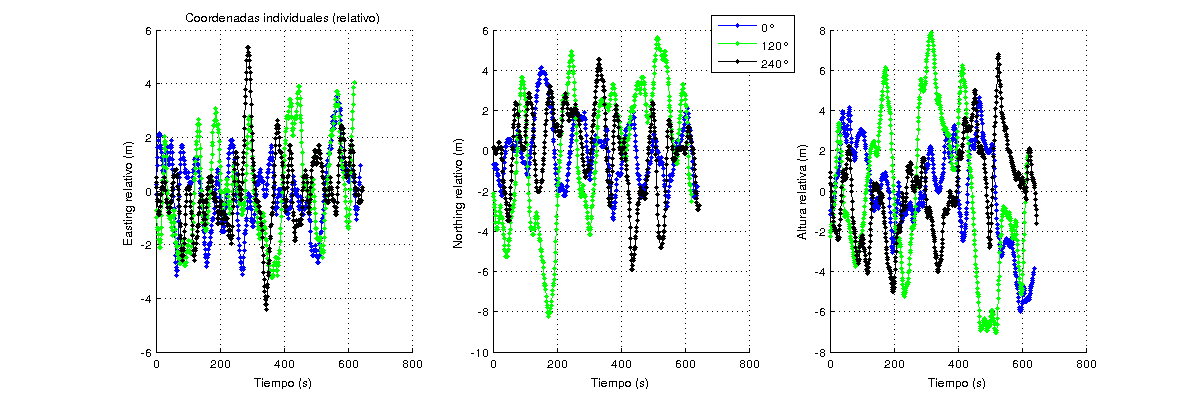
\includegraphics[width=1.4\textwidth]{./pics_gps/orientacion_individual.png}
  \caption{Datos rotando el GPS sobre un punto fijo.}
  \label{fig:orientacion_individual.png}
\end{figure}

\subsubsection{Orientación - Conclusiones}
\label{sec:orientacion-conclusiones}

No se encontró una correlación entre la orientación del GPS y el error en las medidas.
El experimento se realizó con cielo abierto, con una buena geometría, en términos de distribución de satélites. Tal vez en situaciones de visibilidad limitada se podría observar una correlación, ya que si la dirección en la que la antena recibe mejor coincide con el lugar donde hay pocos satélites, entonces la cantidad de información sería menor/peor que en otras orientaciones.

Tener visibilidad limitada por obstáculos, o tener una mala geometría deteriora la performance del GPS. No es el objetivo de este informe evaluar la performance en ambientes complicados.

%El impacto de la geometría se analiza en la sección \ref{sec:geometria}.

\newpage
\subsection{Polígono}
\label{sec:gps2-poligono}

En la figura \ref{fig:10min_pol.png}, la línea en roja representa el polígono resultante de unir el promedio, en cada vértice, de las muestras tomadas durante de 10 minutos. En la figura \ref{fig:10m_mapa.png} se dicho polígono, proyectado sobre una foto satelital\footnote{El mapa y las fotos se obtuvieron de:\\ \url{http://sig.montevideo.gub.uy/mapas/mapa-principal}}.

\begin{figure}[h!]
  \centering
  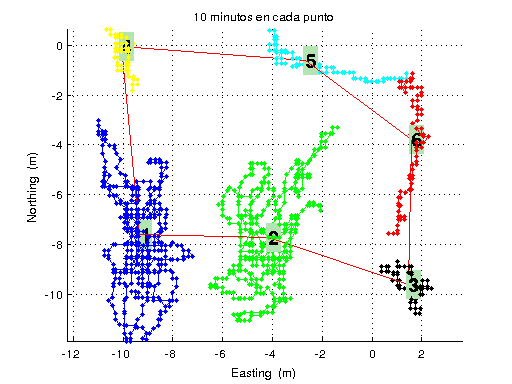
\includegraphics[width=.8\textwidth]{./pics_gps/10min_pol.png}
  \caption{Polígono formado por los promedios de 10 minutos.}
  \label{fig:10min_pol.png}
\end{figure}

\begin{figure}[h!]
  \centering
  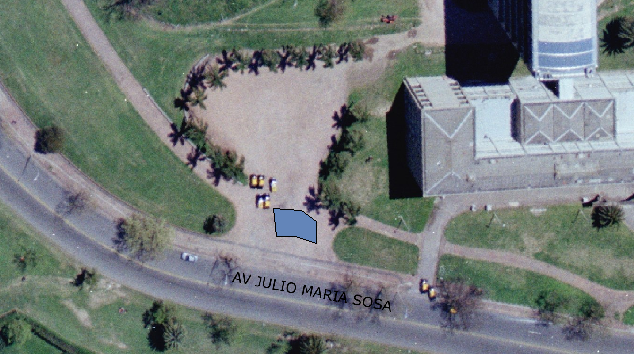
\includegraphics[width=.8\textwidth]{./pics_gps/10m_mapa.png}
  \caption{Proyección del polígono formado por los promedios de 10 minutos sobre una foto satelital.}
  \label{fig:10m_mapa.png}
\end{figure}

En las siguientes figuras se observan los polígonos formados por los promedios de varias secuencias de 2 minutos por punto. 

\newpage
\begin{figure}[h!]
  \centering
  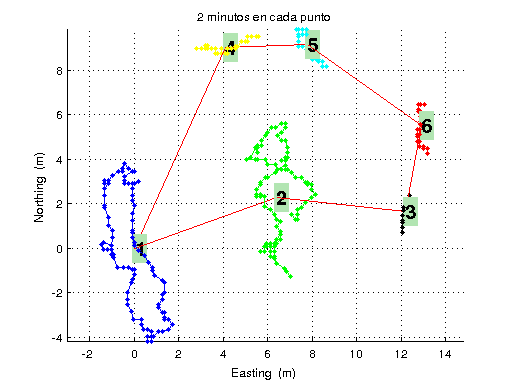
\includegraphics[width=.75\textwidth]{./pics_gps/2m_or1_pol.png}
  \caption{Orientación: \textbf{4}.}
\vspace{-30pt}
  \label{fig:2m_or1_pol.png}
\end{figure}

\begin{figure}[h!]
  \centering
  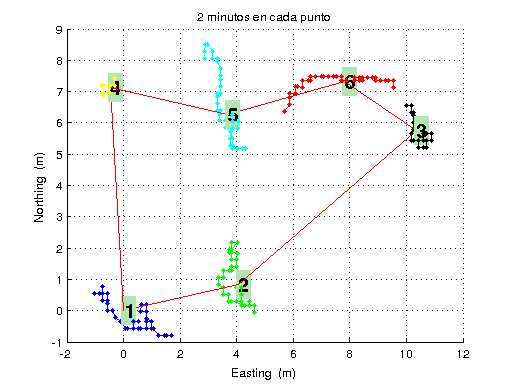
\includegraphics[width=.75\textwidth]{./pics_gps/2m_or2_pol.png}
  \caption{Orientación: \textbf{2}.}
\vspace{-30pt}
  \label{fig:2m_or2_pol.png}
\end{figure}

\newpage
\begin{figure}[h!]
  \centering
  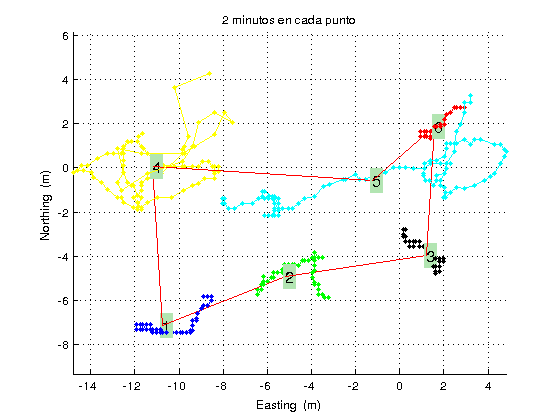
\includegraphics[width=.8\textwidth]{./pics_gps/or2_poly_cut.png}
  \caption{Orientación: \textbf{3}.}
\vspace{-30pt}
  \label{fig:or2_poly_cut.png}
\end{figure}

\begin{figure}[h!]
  \centering
  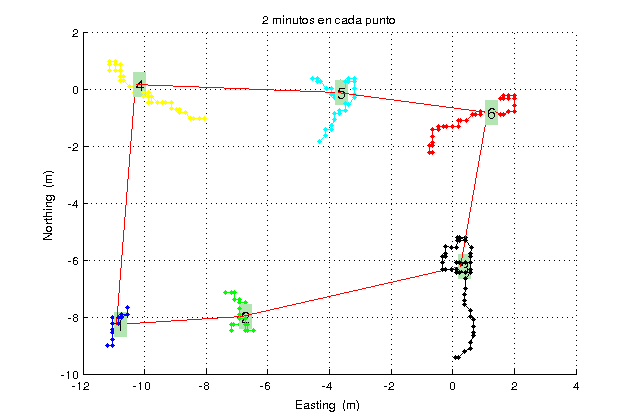
\includegraphics[width=.8\textwidth]{./pics_gps/or3_pol.png}
  \caption{Orientación: \textbf{4}}
  \label{fig:or3_pol.png}
\end{figure}

\subsection{Polígono - Análisis}
\label{sec:poligono-analisis}

Dado que no se cuenta con una referencia absoluta, como podría serlo un GPS de alto nivel, no es posible hablar de error absoluto. De cualquier forma, con la información disponible es posible obtener un estimador del error típico en una distancia de \verb+X+ metros, donde \verb+X+ pertenece al conjunto de las medidas de las rectas en juego: \verb+{6;8.5;12;13.45}+ metros. Se comparan las distancias entre los vértices del polígono experimental, con las distancias entre las coordenadas resultantes de la aplicación de mínimos cuadrados a las medidas efectuadas con el metro (ver la sección \ref{sec:verificacion-del-poligono}).

El error relativo para cada recta resulta:

\begin{equation}
  \label{eq:gps-err-rel}
  E = \left|\|\hat{P}_{i} - \hat{P}_{j}\| - D_{ij}\right|
%  E = \frac{1}{N}\sum_{i=1}^{5}\sum_{j=i+1}^6\left|\|\hat{P}_{i} - \hat{P}_{j}\| - D_{ij}\right|
\end{equation}

Donde:
\begin{itemize}
\item $\hat{P}_i$ es la dupla \verb+{x,y}+, coordenadas experimentales del i-ésimo vértice del polígono.
\item $D_{ij}$ es la distancia entre el i-ésimo y el j-ésimo vértice, resultado de la aplicación de MC en la sección \ref{sec:verificacion-del-poligono}.
\end{itemize}

Para cada set de estimaciones de la posición de los vértices del polígono\footnote{Un set de valores $\hat{P}_1^1,\hat{P}_2^1,\hat{P}_3^1,\hat{P}_4^1,\hat{P}_5^1,\hat{P}_6^1$}, se utilizó la fórmula \ref{eq:gps-err-rel}, separando los datos según el largo esperado de la recta\footnote{Valores posibles: \{6;8.5;12;13.45\}}. Resulta un set de valores del ``\textit{error al estimar la distancia entre dos puntos que deberían estar a X metros}'', para cada valor de \verb+X+. 

Los resultados se resumen en la tabla \ref{tab:err-rectas}.

\begin{table}[H]
\begin{center}
\begin{tabular}{|p{65pt}|c|c|c|c|}
\hline
\textbf{Largo Teo. (cm)} & $\mu$ (cm) & $\sigma$ (cm)  & $\frac{\mu + 2\sigma}{\text{Largo Teo.}}$ & \textbf{\# Muestras} \\
\hline
\rowcolor[gray]{0.9}
600 & 372.15 & 169.39 & 118\% & 35\\
\hline
\rowcolor[gray]{0.8}
848 & 493.6 & 165.79 & 97\%& 20\\
\hline
\rowcolor[gray]{0.9}
1200 & 429.67 & 212.81 & 71\% & 10\\
\hline
\rowcolor[gray]{0.8}
1341 & 614.73 & 166.71 & 70\% & 10\\
\hline
\end{tabular}
\caption{}
\label{tab:err-rectas}
\end{center}
\end{table}

En la tabla \ref{tab:err-rectas} se observa, cómo es de esperarse, que el error relativo disminuye al intentar estimar distancias mayores. Asumiendo que el error en la estimación de la posición de cada punto \verb+A+, \verb+B+ es similar, entonces para cometer un error de \verb+P+\% en la estimación de una distancia \verb+X+ (medida con el metro) entre \verb+A+ y \verb+B+, el GPS debe equivocarse en $\frac{P}{100}X\frac{1}{2}$ en la estimación de la posición de \verb+A+ y \verb+B+.

Resulta que el error en la estimación de la posición de un punto es de aproximadamente 4.5m. Esto es coherente con los resultados sobre la estimación de un punto fijo. Si las medidas para la posición de un punto fijo en general caen dentro de un círculo de 2.5m de radio, entonces, asumiendo que la posición real cae dentro del círculo, en un peor caso se tendría un error de 5m. 

Nuevamente, no se cuenta con información sobre la posición real, pero parece razonable asumir que la ubicación real es cercana al promedio de los datos provenientes del GPS. Evidencia a favor de esto se observa en la figura \ref{fig:10m_mapa.png}. Se trata este tema un poco más en la sección \ref{sec:posicion-absoluta}.

\newpage
\section{Caminata por el borde del polígono}
\label{sec:caminata-por-el-borde-del-poligono}

Para simular una situación más parecida a la que se tendrá con el GPS montado sobre el cuadricóptero, se colocó el trípode con el GPS en un mochila, y se procedió a recorrer el polígono con con la mochila puesta.

Los errores en la medida de un punto fijo hacen pensar que sería posible que la trayectoria determinada por el GPS luego de este experimento fuese algo parecido a un rectángulo.

En las figuras siguientes se observan los datos tomados durante 3 caminatas siguiendo el contorno del polígono, siguiendo la secuencia \verb+1-2-3-6-5-4-1+\footnote{Notar que \textbf{no} se recorre en el mismo orden en el que se numeran los puntos del rectángulo}. Se empezó a loguear datos en el punto 1, y se terminó nuevamente en el punto 1.

\begin{figure} [h!]
  \centering
  \subfloat[Caminata \#1]{\label{fig:caminata1.png}
  		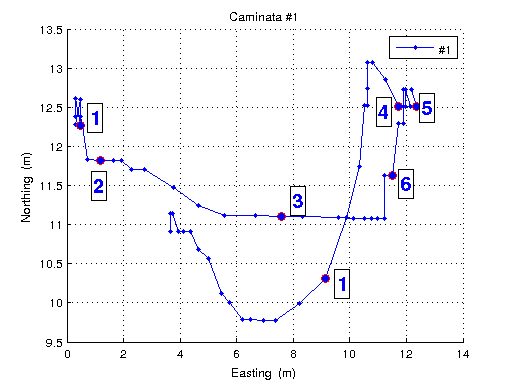
\includegraphics[width=0.55\textwidth]{./pics_gps/caminata1.png}}
  \subfloat[Caminata \#2]{\label{fig:caminata2.png}
  		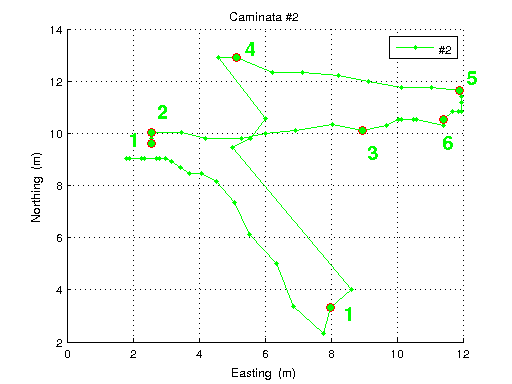
\includegraphics[width=0.55\textwidth]{./pics_gps/caminata2.png}}
  \label{fig:caminatas}
\end{figure}

\begin{wrapfigure}{r}{0.5\textwidth}
  \begin{center}
\vspace{-60pt}
    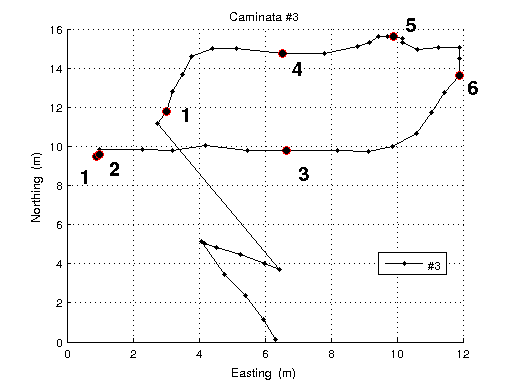
\includegraphics[width=0.5\textwidth]{./pics_gps/caminata3.png}
  \end{center}
  \caption{Caminata \#3}
  \label{fig:caminata3}
\end{wrapfigure}

\subsection{Caminata - Análisis}
\label{sec:caminata-analisis}

Las gráficas de las caminatas a primera vista son muy desalentadoras. Se observa un error que parece ser muy significativo, la trayectoria no se parece en nada a un rectángulo. Un análisis más detallado de los resultados revela que la performance del GPS es acorde a los esperado según las pruebas de las secciones anteriores.

La posición parece tender a estabilizarse una vez que se llega al destino final, el punto 1. Ahí se continuó logueando datos por unos 20 segundos. En la figura \ref{fig:caminata2.png} la posición final parece tener un drift que se aleja de la posición inicial, en lugar de acercarse. No se encontró una justificación para este comportamiento, pero es similar al observado para puntos fijos, por lo que no se le prestó especial atención.

\newpage
\section{Error en altura}
\label{sec:error-en-altura}

Para determinar el error la información sobre la altura que provee el GPS, se diseñó un experimento, que consiste en tomar medidas en una perpendicular a la esfera terrestre, a 4 alturas diferentes: 0m, 1m, 2m y 3m respecto al suelo.

En la primera etapa del experimento, se mantuvo el GPS quieto en cada uno de los niveles, y se tomaron muestras durante aproximadamente 60 segundos. El objetivo de esta etapa era verificar si era viable el experimento.

Se colocó una escalera en el medio del estacionamiento de atrás de la Facultad de Ingeniería, se ató un piolín con marcas cada 1 metro, y una plomada en la punta para mantenerlo tenso y vertical.

\begin{figure}[h!]
  \begin{center}
  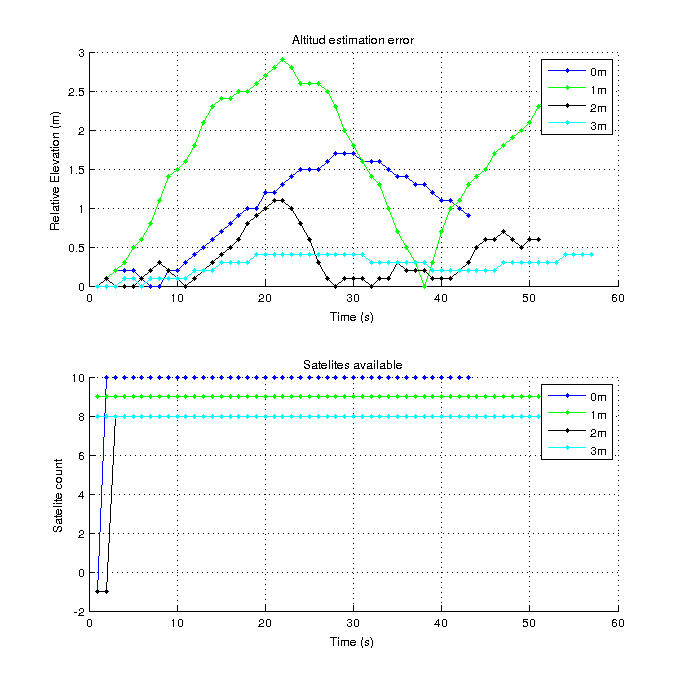
\includegraphics[width=.7\textwidth]{./pics_gps/altura_punto_fijo_fing.png}
  \end{center}
  \caption{Variación de la altura determinada por el GPS a distintas alturas.}
  \label{fig:altura_punto_fijo_fing.png}
\end{figure}

En la figura \ref{fig:altura_punto_fijo_fing.png} se observan los resultados del experimento. Es de esperarse que el error sea mayor al estar apoyado sobre el suelo, ya que los rebotes (\textit{multipath}) pueden deteriorar el sistema. El error a 1m de altura es mayor al que se obtuvo con el GPS en el suelo, una posible explicación para esto sería que el GPS estaba muy cerca de la escalera metálica, lo cual podría introducir una cantidad significativa de rebotes.

Los resultados de este experimento llevan a pensar que el GPS da información estable si se encuentra a al menos 2m del suelo. Esto no parece ser un problema, ya que el cuadricóptero volará a más de 2m de altura.

\newpage
\section{Tiempo de \textit{warmup}}
\label{sec:tiempo-de-warmup}

El tiempo que demora el GPS en adquirir un \textit{fix} depende de si estaba frío, o si estaba andando previamente.
\begin{itemize}
\item \textbf{Frío}: Aproximadamente 40 segundos.
\item \textbf{Caliente}: Entre 3 y 5 segundos.
\end{itemize}

Esto implicaría que al prender el cuadricóptero, habría que esperar unos 40 segundos para obtener señal del GPS, y que si por algún motivo se pierde la conexión con el GPS, habrá que esperar entre 3 y 5 segundo antes de contar con datos útiles nuevamente.

\section{Tasa de muestreo}
\label{sec:tasa-de-muestreo}

El GPS bajo funcionamiento normal trabaja a 1Hz. Se observó que estando quieto, a veces repite información, y la etiqueta como ``válida''. Se observó este comportamiento durante los experimentos de punto fijo, llegando a pasar 30 segundos registrando exactamente la misma información.

Se compararon los datos crudos provenientes del GPS con los que devuelve el GPSD, y se concluyó que el GPSD \textbf{no} es responsable de la repetición de datos, es decir, no es un problema de software, sino que el GPS es el que a veces repite datos.

Al loguear trayectorias de movimiento permanente, como un recorrido en bicicleta de 15 minutos, no se observó más de 4 segundo de corrido de datos repetidos.

No parece razonable que el cálculo de la posición dé \textit{exactamente} lo mismo durante varias medidas sucesivas, probablemente se trate de un problema interno del GPS.

Para enfrentar este problema, lo más razonable parece ser que el algoritmo que lea datos del GPS ignore datos repetidos.

\newpage
\section{Posición Absoluta}
\label{sec:posicion-absoluta}

No se cuenta con fuente de información que nos permite saber exactamente donde estaba el GPS al momento de tomar datos. Se podría haber usado un GPS de mejor calidad como referencia, aunque la performance de los GPS comerciales de un costo razonable no suele ser mucho mejor que la que se obtuvo en los experimentos realizados.

\begin{wrapfigure}{r}{0.7\textwidth}
  \begin{center}
\vspace{-30pt}
  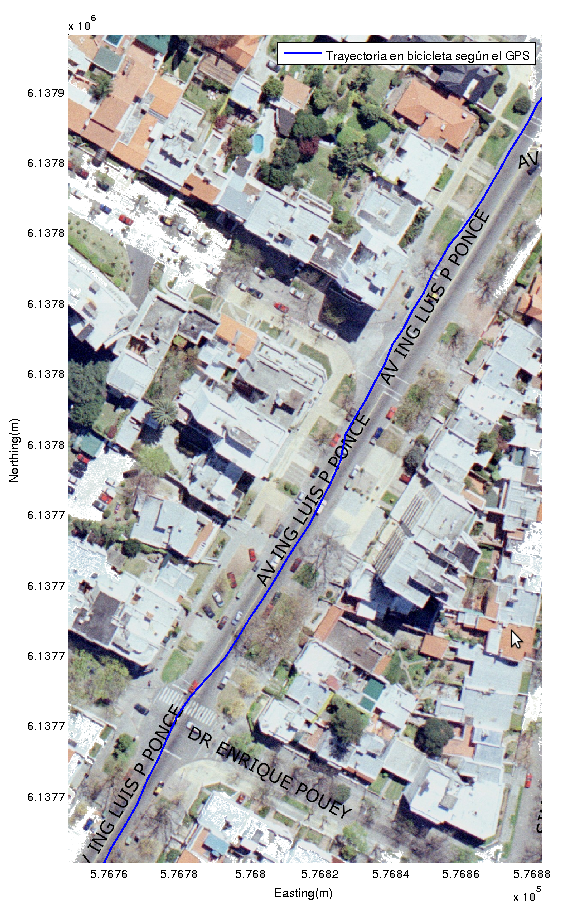
\includegraphics[width=.8\textwidth]{./pics_gps/ponce.png}
  \end{center}
  \caption{Recorrido en bicicleta.}
  \label{fig:ponce.png}
\end{wrapfigure}


Se realizaron varios experimentos para analizar si la ubicación que daba el GPS se correspondía con la realidad, ya que algunos GPSs a veces dan un error constante de varios metros, y de ser el caso, se podría compensar este problema una vez detectado.

Sobre un mapa de Montevideo, se graficaron trayectorias conocidas, con el objetivo de verificar que los datos provenientes del GPS eran ``razonables''.

No se observo un offset evidente y constante, por lo que se asume el GPS \textbf{no} introduce un offset, o por lo menos no una constante, que se pueda compensar corriendo todos los datos por una cantidad fija.

En la figura \ref{fig:ponce.png} se observa una trayectoria realizada en bicicleta, con el GPS colocado sobre el trípode, asomando de una mochila. El recorrido fue hacia el sur-oeste, sobre la senda derecha, contra el lado derecho (cerca del cordón). No se observa un offset constante. Se analizaron otras figuras, y se llegaron a conclusiones similares.

\newpage
\section{Conclusiones}
\label{sec:conclusion}

Los siguientes items servirán de guía para la utilización del GPS como instrumento de navegación:

\begin{itemize}
\item \textbf{Error en las medidas}: Bajo las condiciones anteriores, se concluye que es razonable asumir que las medidas del GPS tienen un \textbf{error menor a 5m}. Esto es un poco menor a las especificaciones dadas por el fabricante del GPS, 5m \emph{CEP}\footnote{\textit{CEP} de Xm: Garantiza que el 50\% de la muestras caerán en un círculo de radio X y centro el promedio de las muestras.}. Es de esperarse que la performance se reduzca al utilizar el GPS en un entorno más agresivo, como el que resultará al colocar el GPS sobre el cuadricóptero, donde estará sujeto a  interferencia electromagnética de los motores, vibraciones, etc.
\item \textbf{Visibilidad}: Es importante asegurar buena visibilidad, la performance del GPS se reduce drásticamente si pierde satélites.
\item \textbf{Promedios}: Promedios de 2 minutos son suficientes para reducir el error a 2.5m, con una probabilidad del 75\%.
\item \textbf{Resolución}: El GPS \textbf{no} es adecuado para tareas de navegación con restricciones del orden del metro, pero sí para distancias del orden de decenas de metros.
\item \textbf{Tasa de muestreo}: El GPS normalmente muestrea a \textbf{1Hz}. Cabe destacar que debe ignorarse información repetida (muestras sucesivas que sea idénticas).
\item \textbf{Error en altura}: El GPS \textbf{no} es adecuado para determinar la elevación durante el aterrizaje/despegue, ya que a menos de 2m del piso, la estimación de la elevación es muy mala. Será necesario otro sensor (sensor de presión, IR, etc) para asistir durante el despegue/aterrizaje.
\item \textbf{Tiempo de \textit{fix}}: En frío demora alrededor de 40 segundos, en caliente entre 3 y 5 segundos.
\end{itemize}

Por último, cabe destacar que los resultados de este informe dan una idea de la performance del GPS en condiciones ``ideales''. Será importante analizar el efecto de las vibraciones y la interferencia electromagnética que introducirá la presencia del cuadricóptero, de manera de ajustar los márgenes de error al contexto en el que se utilizará el GPS.

\end{document}